\shorthandoff{"}
\chapter{Diskussion}
\label{ch:diskussion}

\section{Zusammenfassung der Forschungsergebnisse}
\label{ch:diskussion:zusammenfassung}
Im Rahmen der vorliegenden Master-Thesis wurde eine Fallstudie durchgeführt, über welche die Vorschläge zur Besetzung offener Projektpositionen eines unilateralen und eines bilateralen Empfehlungsansatzes miteinander verglichen wurden. Dabei konnte das bilaterale Vorschlagsverfahren bei vier der fünf evaluierten Stellen eine höhere Zufriedenheit bei den Angestellten erzielen. Bei einer Projektposition sorgte dagegen der unilaterale Empfehlungsansatz für eine höhere Zufriedenheit. Vergleichbar fielen auch die Ergebnisse auf Seiten der Projektmanager aus. Hier prognostizierten die Verantwortlichen für drei der fünf Stellen eine höhere Arbeitsleistung von den vorgeschlagenen Mitarbeitern des bilateralen Empfehlungsansatzes. Bei zwei Projektpositionen bewerten die Projektmanager dagegen die Arbeitsleistungen der Vorschläge der unilateralen Variante als höher.

Bei grafischer Darstellung von Präferenzen und beherrschten Fähigkeiten zeigte sich der sogenannte lange (Ratten-)Schwanz für die befragten Mitarbeiter der EXXETA AG. Bezüglich der in den vordefinierten Projektpositionen benötigten Kompetenzen konnte festgestellt werden, dass die Mitarbeiter einen Großteil ihrer präferierten Kompetenzen noch nicht beherrschen. Außerdem ist der Anteil an Mitarbeitern, welche eine gesuchte Fähigkeit beherrschen und gleichzeitig präferieren und der Anteil an Angestellten, welche nicht über eine benötigte Kompetenz verfügen und diese dennoch präferieren, im Durchschnitt gleich groß. Darüber hinaus gaben knapp über 40 Prozent aller Mitarbeiter eine Fähigkeit nicht als Präferenz an, obwohl sie diese beherrschen. Weitere Analysen ergaben, dass 17 Prozent der befragten Mitarbeiter keine einzige Kompetenzbewertung im Intranet der EXXETA AG vorgenommen hatten.

Abschließend wurde evaluiert, wie Mitarbeiter und Projektmanager mit möglicher Unterforderung bei der Projektarbeit umgehen. Diese Information ist gemäß der Theorie des \acp{PEFit} zur korrekten Berechnung der Kongruenz von Mitarbeitern und Projektposition notwendig. Im Rahmen der Befragung konnte hierbei festgestellt werden, dass sowohl Projektmanager als auch Mitarbeiter mehrheitlich eine Unterforderung vermeiden möchten.

\section{Interpretation der Forschungsergebnisse}
\label{ch:diskussion:interpretation}
In Kapitel \ref{ch:personEnvironmentFit:auswirkungenErhoehterAngebote} wurde beschrieben, dass ein P-E Misfit in drei möglichen Konsequenzen mit entsprechenden Gleichungen zur Berechnung resultieren kann. Im Rahmen der vorliegenden Master-Thesis wurde angenommen, dass sowohl Projektmitarbeiter als auch -manager eine Unterforderung bei der Besetzung offener Projektpositionen vermeiden möchten. Dementsprechend wurde Kurve B aus Abbildung \ref{fig:personEnvironmentFit:auswirkungenErhoehterAngebote:abb1} in Form der quadrierten Differenzberechnung implementiert. Die in Abbildung \ref{fig:ergebnisse:fallstudie:kurven:abb1} dargestellten Ergebnisse bestätigen diese Annahme sowohl aus Perspektive der Mitarbeiter als auch aus dem Blickwinkel der Projektverantwortlichen. 

Bei Implementierung der beiden Empfehlungsansätze wurde aufgrund der Erkenntnisse aus Kapitel \ref{ch:empfehlungssysteme} erwartet, dass der lange (Ratten-)Schwanz und der Kaltstart die Vorschlagserstellung beeinträchtigen werden. Daher lag beiden Empfehlungsmethoden ein hybrider und graphenbasierter Ansatz zugrunde, welcher über die Einbeziehung von Fähigkeitsbewertungen und Teamzuordnungen beide Probleme löste. Dieses Vorgehen ist mit Blick auf die Ergebnisse in Abbildung \ref{fig:ergebnisse:analyse:abb1} als sinnvoll zu bewerten, da sowohl bei beherrschten als auch präferierten Fähigkeiten ein langer (Ratten-)Schwanz erkennbar ist. Zusätzlich ist Kapitel \ref{ch:ergebnisse:analyse:intranetUndUmfrage} zu entnehmen, dass 17 Prozent der Mitarbeiter im Intranet keine einzige Fähigkeit bewertet hatten und diese ohne Einbeziehung der Teamzuordnungen folglich von einem Kaltstart betroffen wären.

Hinsichtlich der Kompetenzen konnte anhand von Abbildung \ref{fig:ergebnisse:analyse:abb3} außerdem beobachtet werden, dass die Mitarbeiter einen Großteil ihrer präferierten Fähigkeiten nicht beherrschen. Aus diesem Sachverhalt lässt sich schließen, dass die Angestellten bereit sind, in Zukunft weitere Fähigkeiten zu erlernen und diese bei der Projektarbeit anzuwenden. Auf Unternehmensseite könnte dementsprechend der Einsatz weiterer Weiterbildungsangebote evaluiert werden, bei welchen die Mitarbeiter nicht nur bestehende Kompetenzen vertiefen, sondern auch neue Fähigkeiten erlernen können.

Sowohl in Abbildung \ref{fig:ergebnisse:analyse:abb3} als auch in Abbildung \ref{fig:ergebnisse:analyse:abb5} kann beobachtet werden, dass das Beherrschen einer Fähigkeit keinen Rückschluss auf eine entsprechende Präferenz zulässt. Ein unilateraler Empfehlungsansatz würde dennoch sämtliche beherrschten Kompetenzen gleich behandeln. Somit ist davon auszugehen, dass die Angestellten bei Einsatz eines unilateralen Empfehlungssystems für Projektpositionen vorgeschlagen werden, deren gesuchte Fähigkeiten diese zumindest teilweise nicht anwenden möchten. Ein bilaterales System unterscheidet dagegen zwischen präferierten und nicht präferierten Kompetenzen. Da dieser Ansatz gewünschte Fähigkeiten stärker gewichtet, wird sich ein vorgeschlagener Mitarbeiter mit höherer Wahrscheinlichkeit die Anwendung der für die offene Projektposition benötigten Kompetenzen wünschen. Dementsprechend ist eine höhere Zufriedenheit und Motivation bei der Stellenbesetzung zu erwarten. Wie in Abbildung \ref{fig:diskussion:interpretation:abb1} zu erkennen, spiegelt sich diese Annahme in den Ergebnissen der Umfragen unter den Projektmitarbeitern und -managern der EXXETA AG wider.

\begin{figure}[h]
	\centering
	
	\subfloat[Prognostizierte Zufriedenheit der Mitarbeiter mit den Beispielprojektpositionen]{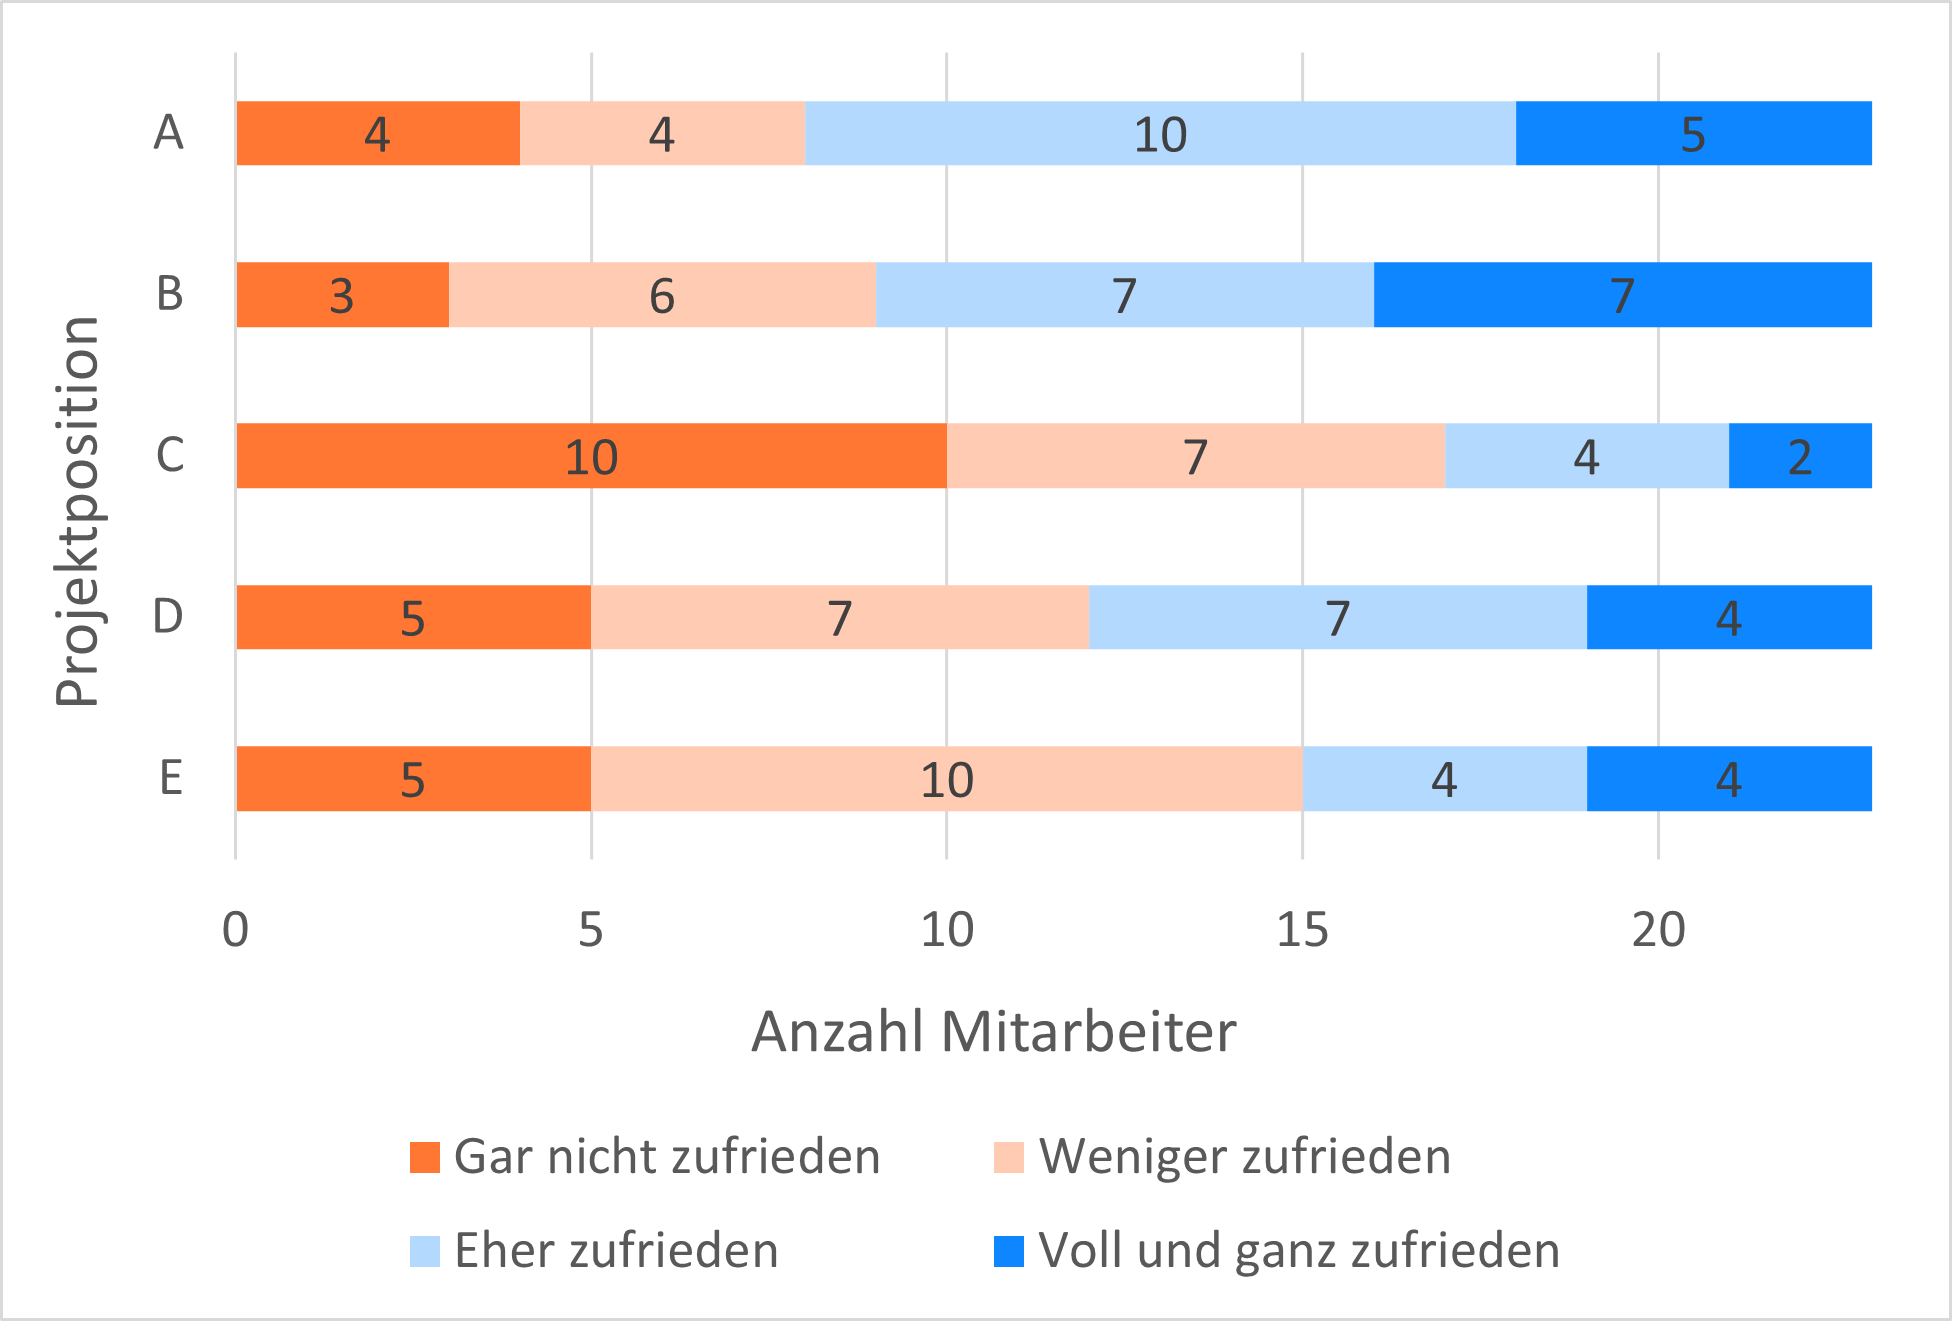
\includegraphics[width = 0.75\textwidth]{gfx/mitarbeiter-zufriedenheit-umfrage.png}}\\
	\subfloat[Ergebnisse Mitarbeiter]{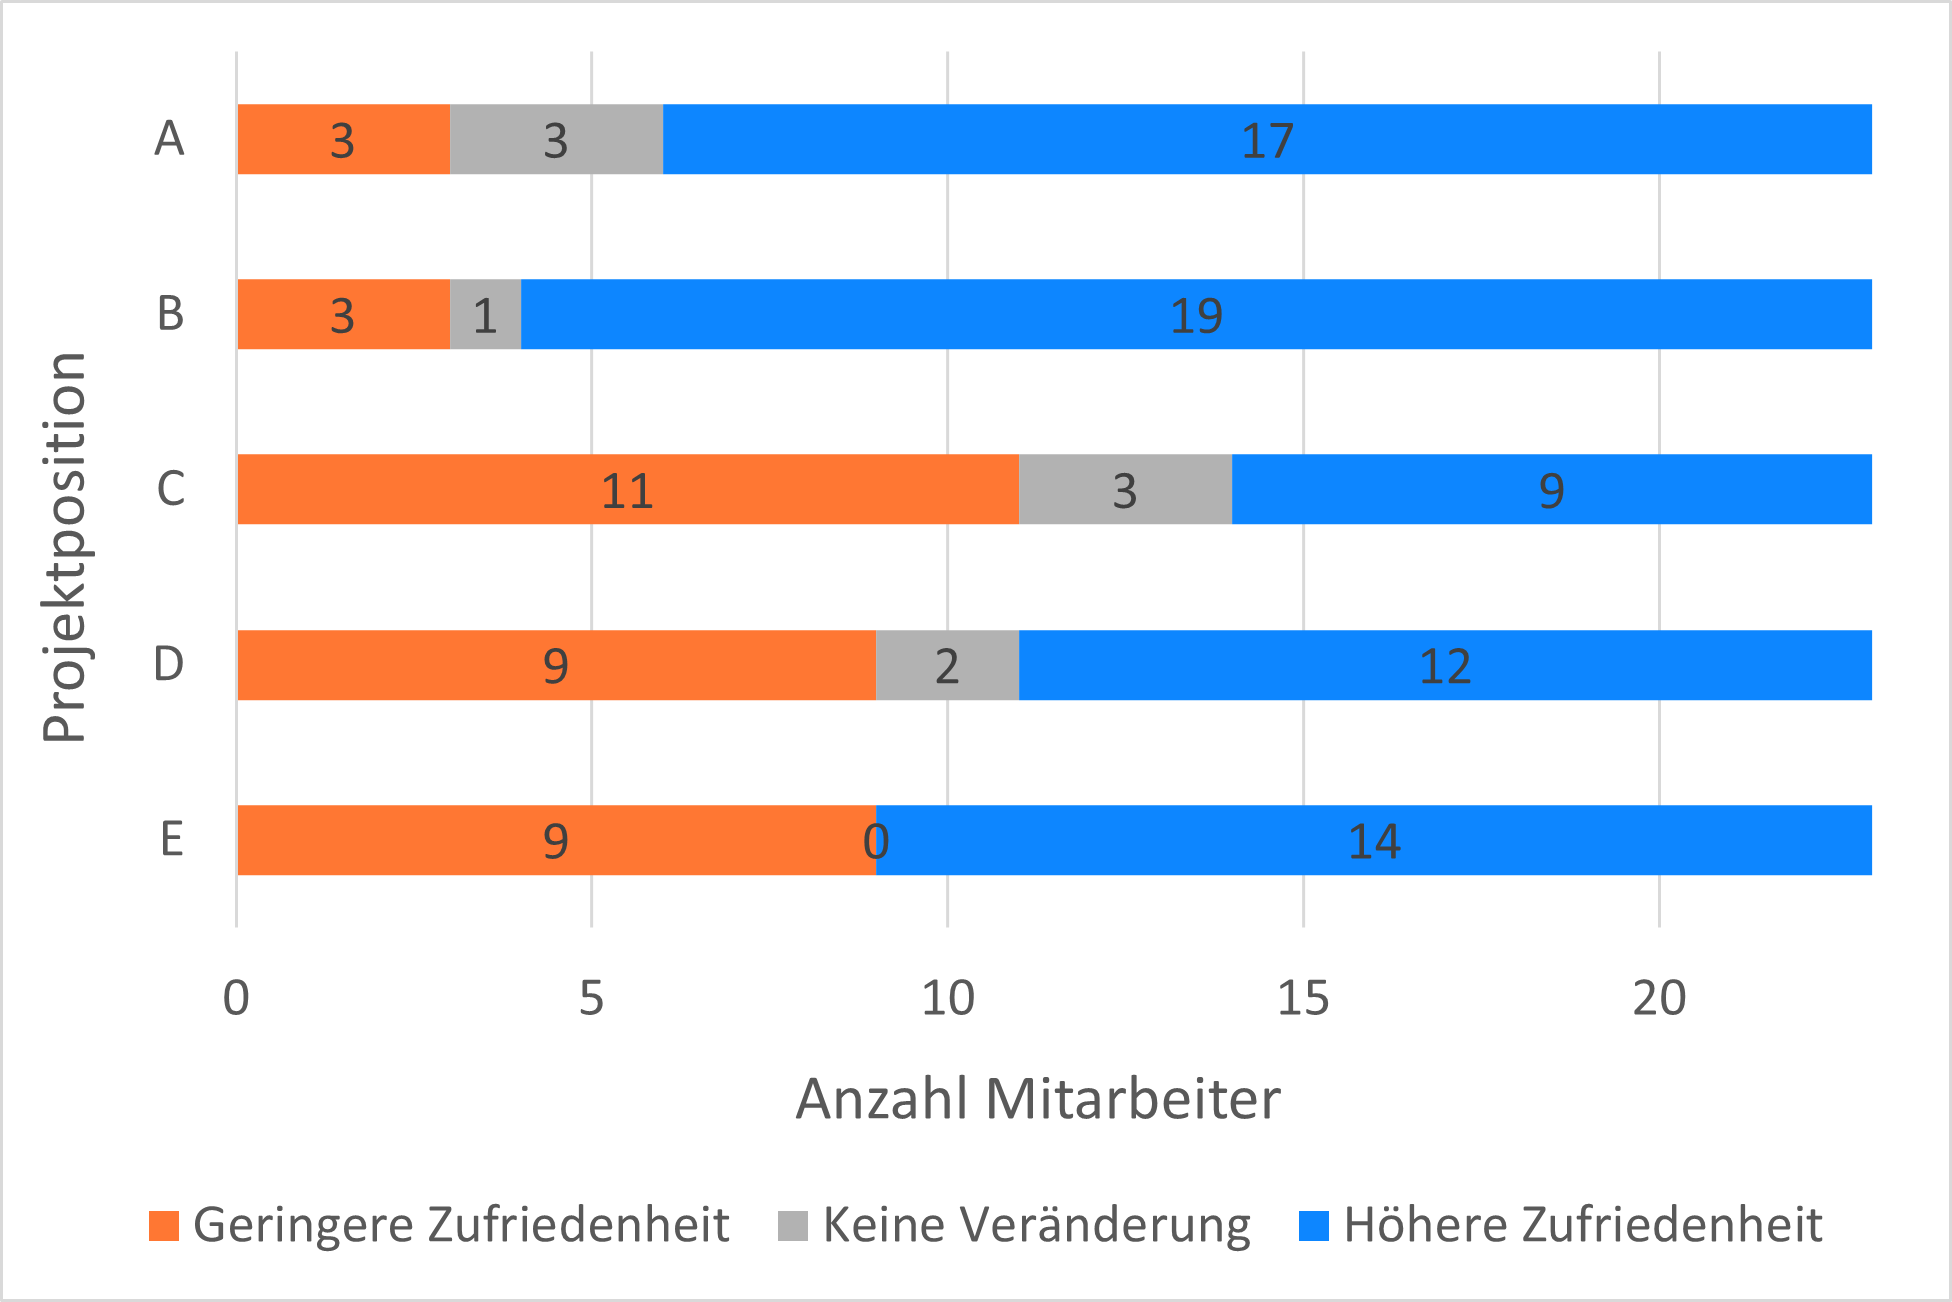
\includegraphics[width = 0.5\textwidth]{gfx/zufriedenheit-projekte.png}}
	\subfloat[Ergebnisse Projektmanager]{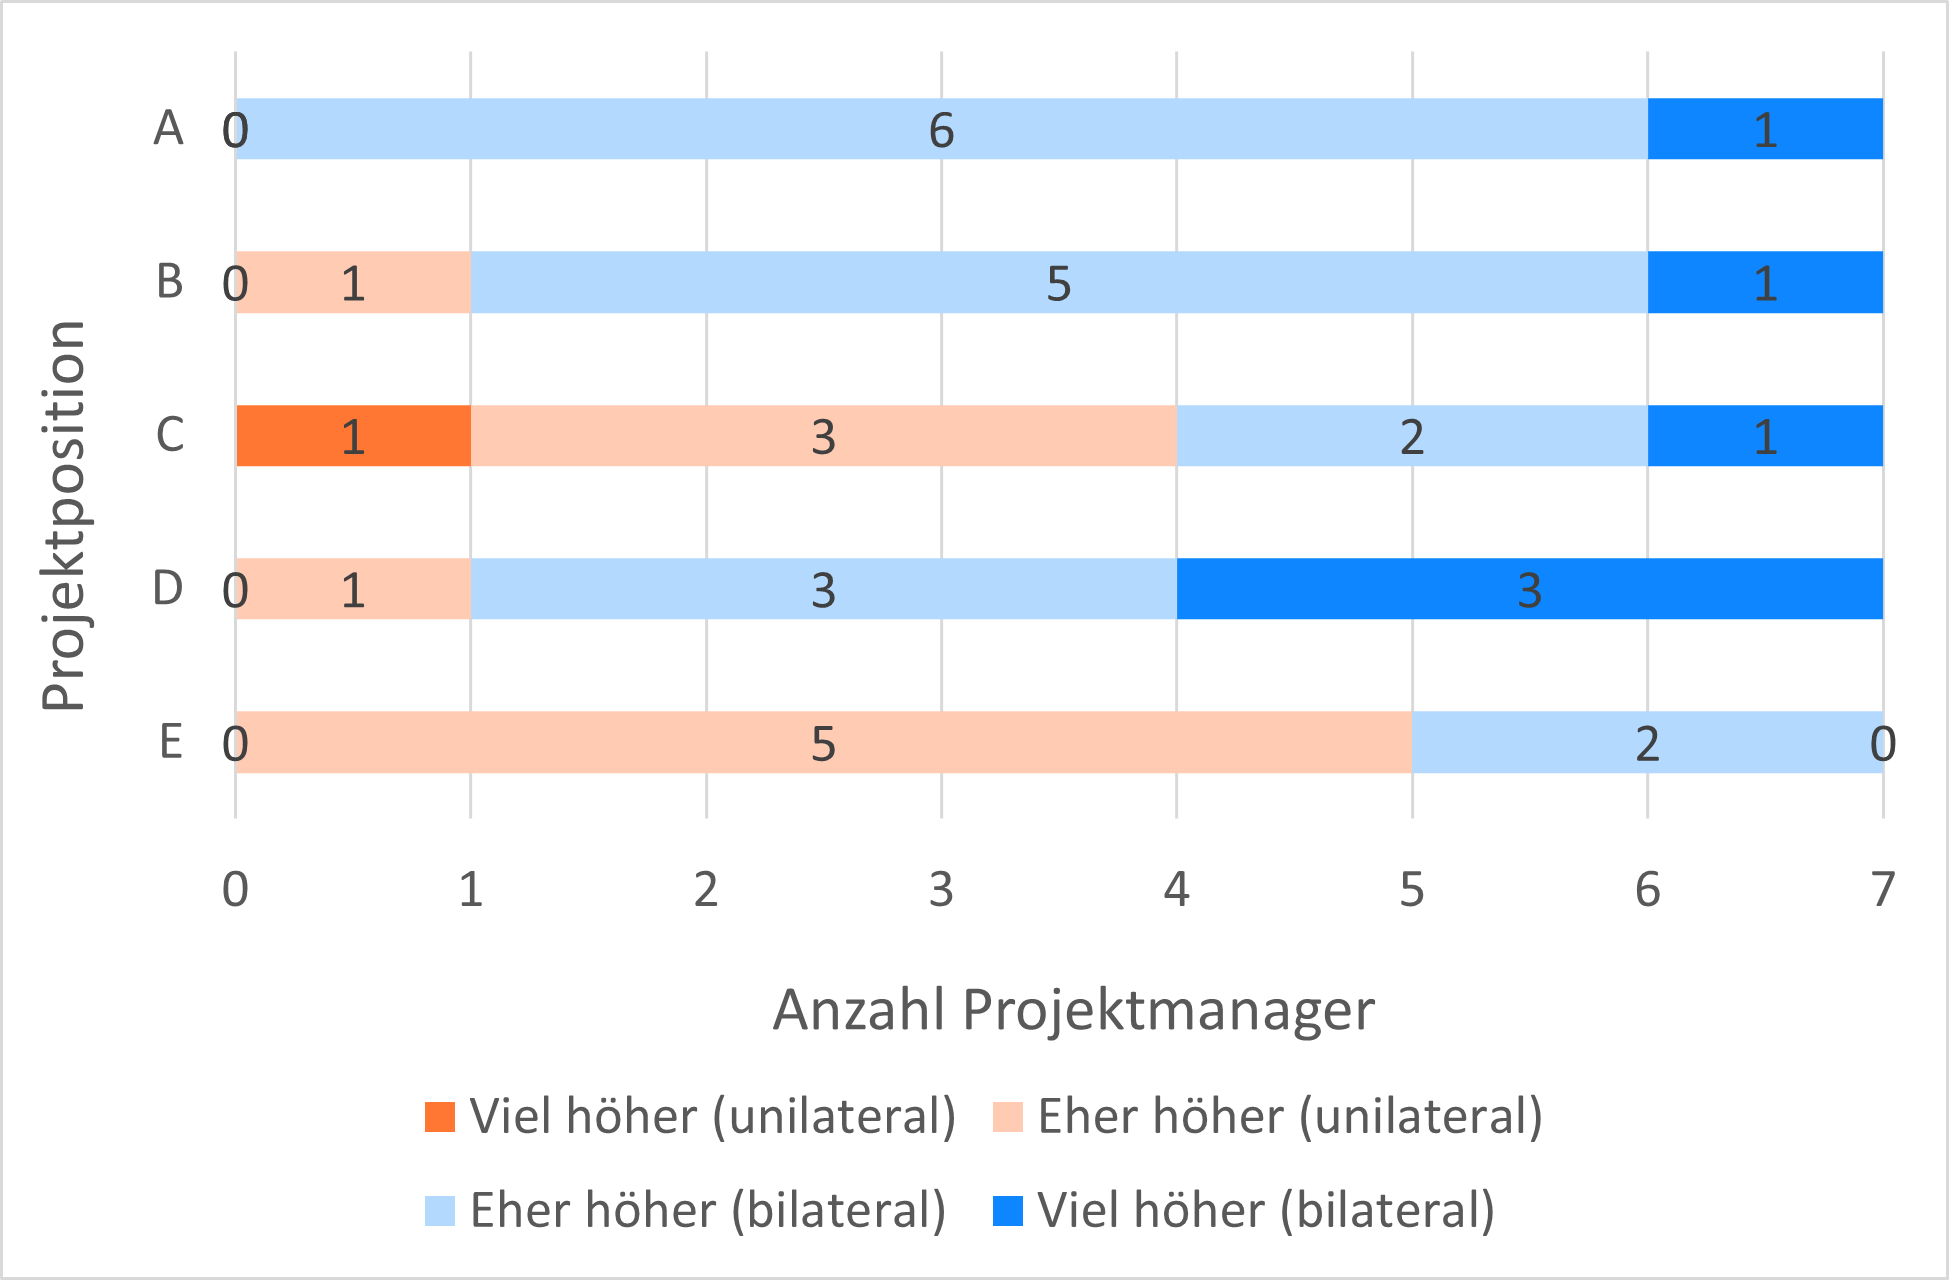
\includegraphics[width = 0.5\textwidth]{gfx/ergebnisse-projektmanager-arbeitsleistung.png}}
	
	\caption{Darstellung der Ergebnisse der Umfragen unter Mitarbeitern und Projektmanagern}
	\label{fig:diskussion:interpretation:abb1}
\end{figure}

An den in Abbildung \ref{fig:diskussion:interpretation:abb1} dargestellten Ergebnissen der Fallstudie ist zu erkennen, dass die Mitarbeiter durch den bilateralen Empfehlungsansatz stärker zu deren Zufriedenheit positioniert werden, wenn sie gleichzeitig eine hohe Zufriedenheit mit der Stelle prognostizieren. Dieser Sachverhalt ist insbesondere bei den Projektpositionen A und B zu beobachten, mit welchen sich über die Hälfte der Mitarbeiter zufrieden zeigen. Hier ordnet der bilaterale Empfehlungsansatz etwa dreiviertel aller Angestellten stärker zu deren Zufriedenheit an, als die unilaterale Methode. Zeigen sich dagegen weniger Mitarbeiter mit einer betrachteten Projektposition zufrieden, nimmt auch die Qualität des bilateralen Empfehlungsansatzes hinsichtlich der Mitarbeiterzufriedenheit ab. Besonders gut ist dieser Sachverhalt bei Projektposition C zu erkennen, mit welcher sich die Mitarbeiter mehrheitlich unzufrieden zeigen. Hier erzielt der bilaterale Empfehlungsansatz im Vergleich zur unilateralen Variante sogar Ergebnisse, welche zu einer geringeren Zufriedenheit der Mitarbeiter führen.

Ähnliche Ergebnisse können aus Abbildung \ref{fig:diskussion:interpretation:abb1} ebenfalls für die Perspektive der Projektmanager abgeleitet werden. Auch hier ist für die Projektpositionen A und B zu beobachten, dass die Verantwortlichen eine höhere Arbeitsleistung von den Vorschlägen des bilateralen Ansatzes erwarten. Für die Projektpositionen C und E, mit welchen sich die Mitarbeiter mehrheitlich unzufrieden zeigen, erwarten die Projektmanager dagegen eine höhere Leistung von den Vorschlägen des unilateralen Empfehlungsansatzes. Eine Ausnahme bildet Projektposition D in Abbildung \ref{fig:diskussion:interpretation:abb1}. Hier sorgen die Vorschläge des bilateralen Empfehlungsansatzes aus Perspektive der Projektmanager für eine wesentlich höhere prognostizierte Arbeitsleistung. Die Erwartungen der Angestellten hinsichtlich ihrer Zufriedenheit mit der Stelle sind dabei sehr ausgeglichen. Wie in Abbildung \ref{fig:diskussion:interpretation:abb2} zu erkennen, unterschieden sich die Vorschläge zu Projektposition D in der Umfrage unter den Projektmanagern in nur einer Person. Aus diesem Grund werden die Ergebnisse der Projektverantwortlichen im vorliegenden Fall als nicht repräsentativ betrachtet.

\begin{figure}[h]
	\centering
	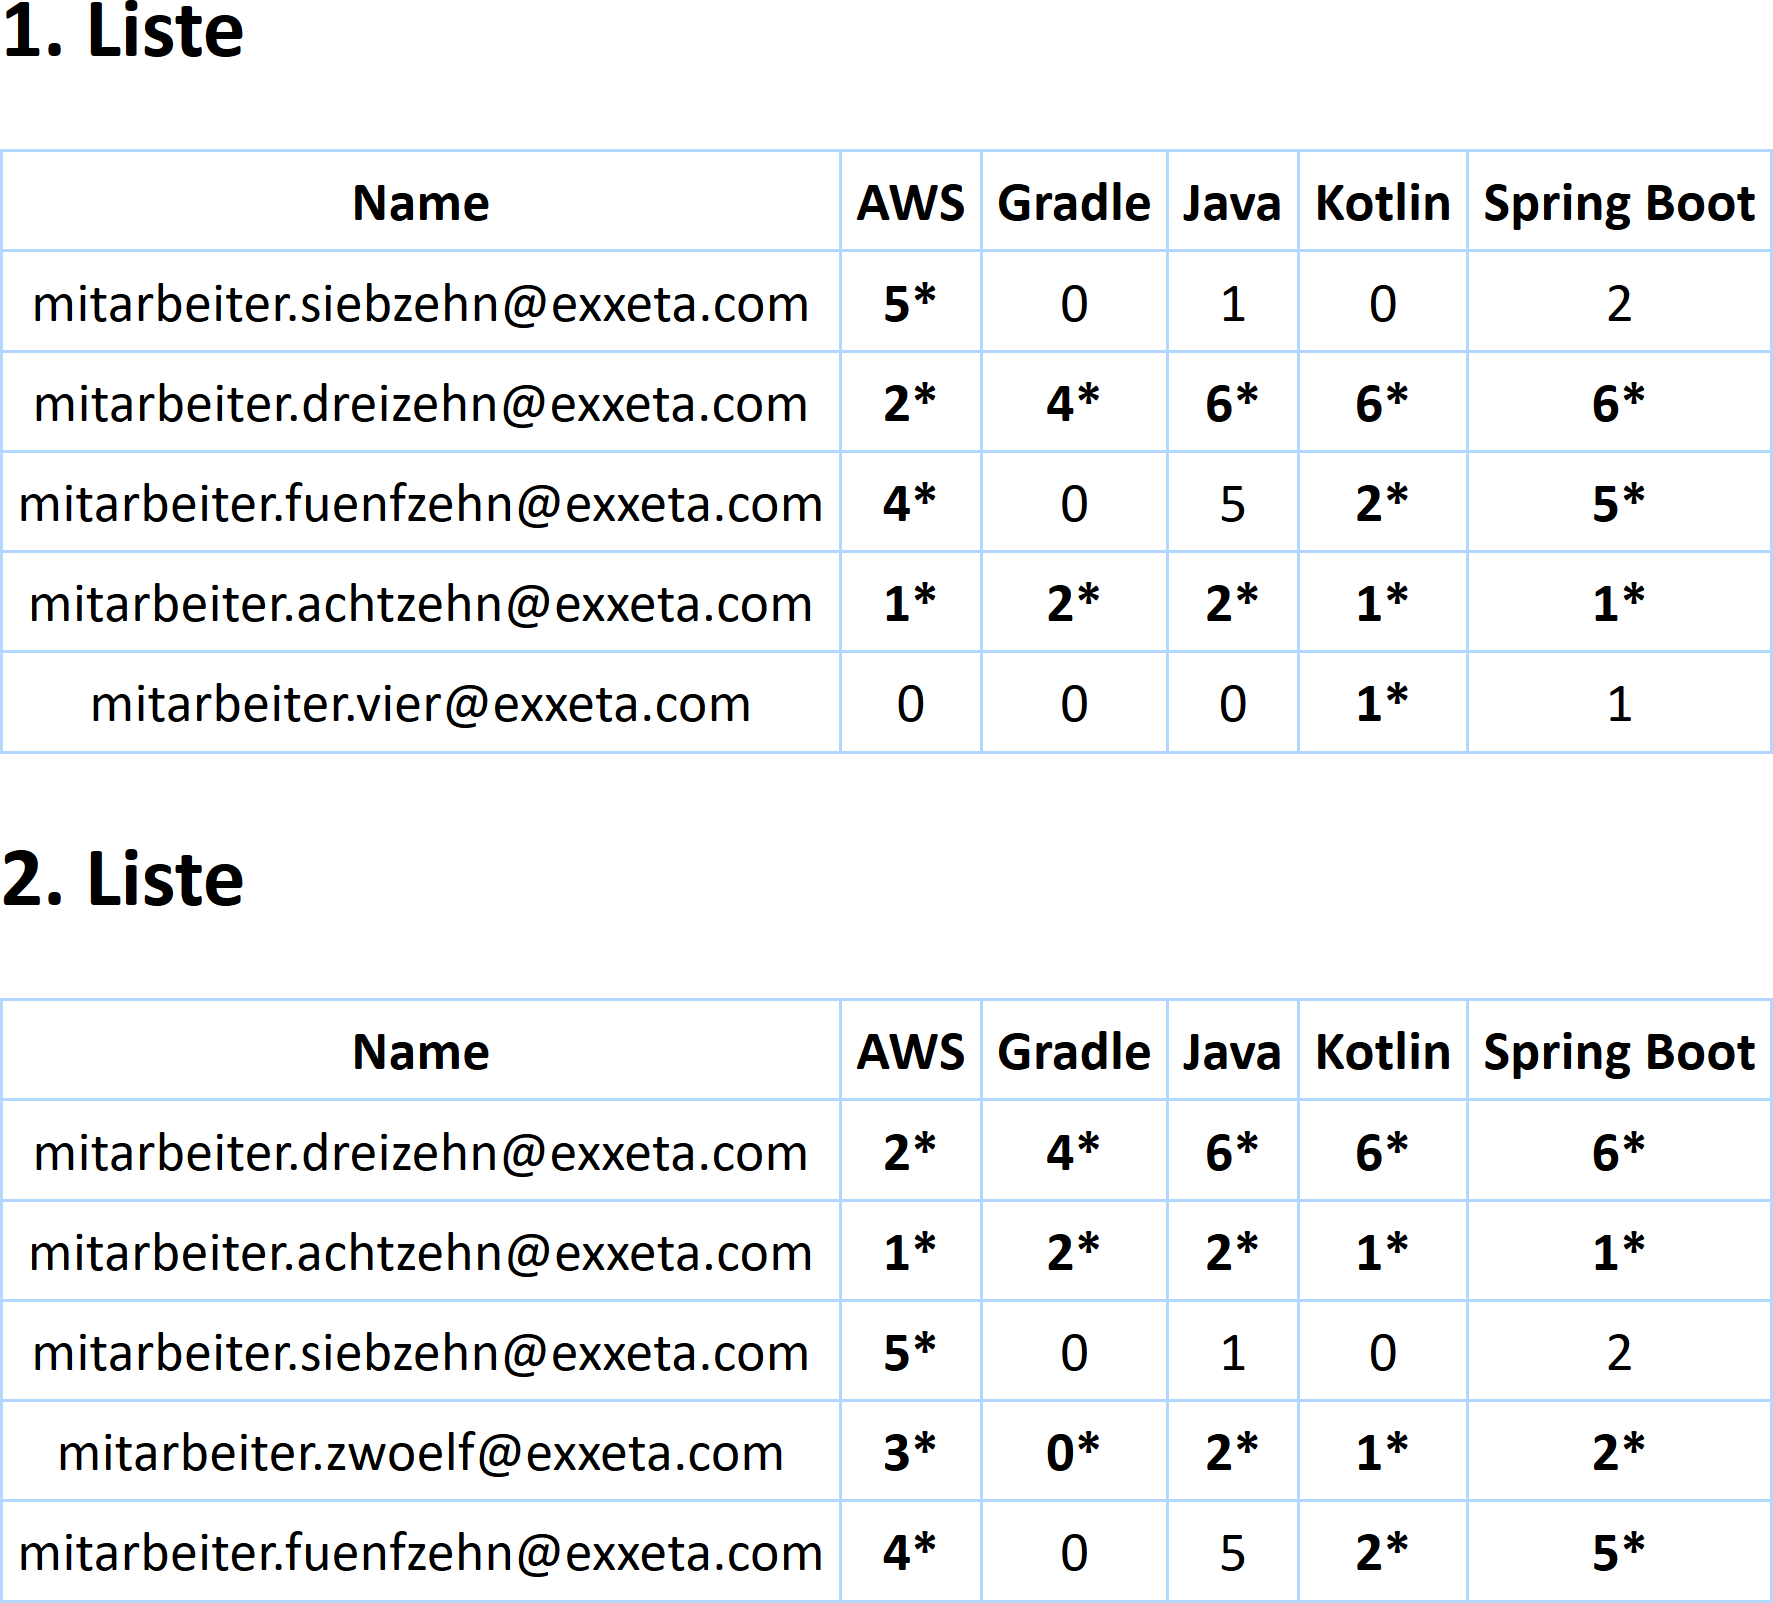
\includegraphics[width=0.75\textwidth]{gfx/projektposition-d.png}
	\caption{Mitarbeiter-Vorschläge für Projektposition D in der Umfrage unter den Projektmanagern\\
	(Klarnamen wurden aus Datenschutzgründen nachträglich pseudonymisiert)}
	\label{fig:diskussion:interpretation:abb2}
\end{figure}

\section{Beantwortung der Forschungsfrage}
\label{ch:diskussion:beantwortungForschungsfrage}
Die vorliegende Master-Thesis verfolgte das Ziel, die folgende Forschungsfrage zu beantworten: \forschungsfrage

Aufgrund der Erkenntnisse aus Kapitel \ref{ch:diskussion:interpretation} ist zur Beantwortung dieser Forschungsfrage festzustellen, dass die Anwendung eines bilateralen Empfehlungssystems bei der Besetzung offener Projektpositionen gleichzeitig die Zufriedenheit der Angestellten und die von den vorgeschlagenen Mitarbeitern erwartete Arbeitsleistung seitens der Projektmanager steigert. Diese Antwort gilt jedoch nur unter der Bedingung, dass sich die Mitarbeiter mehrheitlich zufrieden mit der betrachteten Projektposition zeigen.

Als Ursache für diese Einschränkung wird die Art der Erhebung der Präferenzen betrachtet. Die Mitarbeiter gaben im Rahmen dieser Master-Thesis ihre Wünsche über boolesche Werte an. Hierbei gewichtete das bilaterale Empfehlungssystem die Fähigkeiten der Angestellten höher, wenn sie diese präferieren. Es wurde jedoch nicht unterschieden, ob ein Angestellter einer nicht gewünschten Kompetenz neutral gegenüber steht oder ob er diese nicht bei der Projektarbeit anwenden möchte.

\section{Empfehlung für weiterführende Forschungen}
\label{ch:diskussion:empfehlung}
Aufgrund der in Kapitel \ref{ch:diskussion:beantwortungForschungsfrage} beschriebenen Einschränkungen der Forschung wird für folgende Arbeiten empfohlen, den im Rahmen dieser Arbeit implementierten Empfehlungsansatz zu erweitern. Hierbei sollten die Präferenzen nicht über boolesche Werte, sondern über Abstufungen der Form "möchte ich anwenden", "neutral", "möchte ich nicht anwenden" erhoben werden.

Bei der Implementierung sollten die Mitarbeiter bei vorhandenem Wunsch weiterhin höher positioniert werden. Bei Angabe der negativen Präferenz sollten die Angestellten jedoch zusätzlich niedriger einsortiert werden. Unter Betrachtung dieser Veränderungen sollte die Evaluation unter Mitarbeitern und Projektmanagern erneut durchgeführt und die Forschungsfrage entsprechend untersucht werden.

\section{Einordnung in die Literatur und Ausblick}
\label{ch:diskussion:einordnung}
Die vorliegende Master-Thesis bestätigt die Hypothese von \textcite{malinowski:2008}, dass das Konzept des \acp{PEFit} bei der Implementierung von Empfehlungssystemen zur Personalauswahl berücksichtigt werden sollte. Sofern die Angestellten eine hohe Zufriedenheit mit einer Projektposition prognostizieren, führt der Einsatz der im Rahmen dieser Arbeit implementierten bilateralen Recommender Engine im Vergleich zu einer unilateralen Variante auf Seiten der Mitarbeiter zu einer höheren Zufriedenheit und erhöht gleichzeitig die erwartete Arbeitsleistung auf Seiten der Projektmanager. Dementsprechend sollten Autoren zukünftiger Publikationen beachten, dass die Optimierung eines Ergebnisses gemäß des \acp{PEFit} nur durch gemeinsame Betrachtung von Person und Umgebung erfolgen kann. Während bisherige Publikationen laut \textcite{malinowski:2008} zumeist entweder die Perspektive von Personalsachbearbeiten bzw. Projektmanagern oder die Sichtweise von Mitarbeitern einnahmen, sollten zukünftige Arbeiten daher verstärkt den Fokus auf die weitere Erforschung bilateraler Anwendungen richten.
\shorthandon{"}